%%%%%%%%%%%%%%%%%%%%%%%%%%%%%%%%%%%%%%%%%%%%%%%%%%%%%%%%%%%%%%%%%%%%%%
%%                    Assignment
%%%%%%%%%%%%%%%%%%%%%%%%%%%%%%%%%%%%%%%%%%%%%%%%%%%%%%%%%%%%%%%%%%%%%%
%\color{blue}

\subsubsection{Glyph: \glyph{Assignment}}\label{sec:assignment}

\glyph{Assignment} is used to describe the setting of a state variable to a certain value. The assignment, represented by an harpoon arrow, goes from one or more \glyph{variable values} to a variable identification, represented by a \glyph{state variable} attached to the entity affected by the assignment. If an \glyph{assignment} takes several \glyph{variable values} as input, there is an implicit XOR between them, located at the point of junction between the arcs coming from the alternative values. Since only one value can be assigned at a time, there is therefore no edge overlap in the assignment itself. The result of an assignment is represented by \glyph{outcomes}, that is by filled dots on the arrow. The result of an \glyph{assignment} can be represented by any number of \glyph{outcomes}. In the case of more than one \glyph{variable values}, the \glyph{outcomes} must be placed on the relevant incoming branch.

\begin{glyphDescription}
 \glyphSboTerm SBO:0000464 ! state variable assignment
 \glyphOrigin One or more variable value (section \sect{variableValue}) on their own, each containing a variable value.
 \glyphTarget A state-variable (section \sect{stateVariable}) carried by an entity (section \sect{entity}), containing a variable identification.
 \glyphEndPoint The target extremity of an \glyph{assignment} carries an harpoon arrowhead.
 \end{glyphDescription}

\begin{figure}[H]
  \centering
  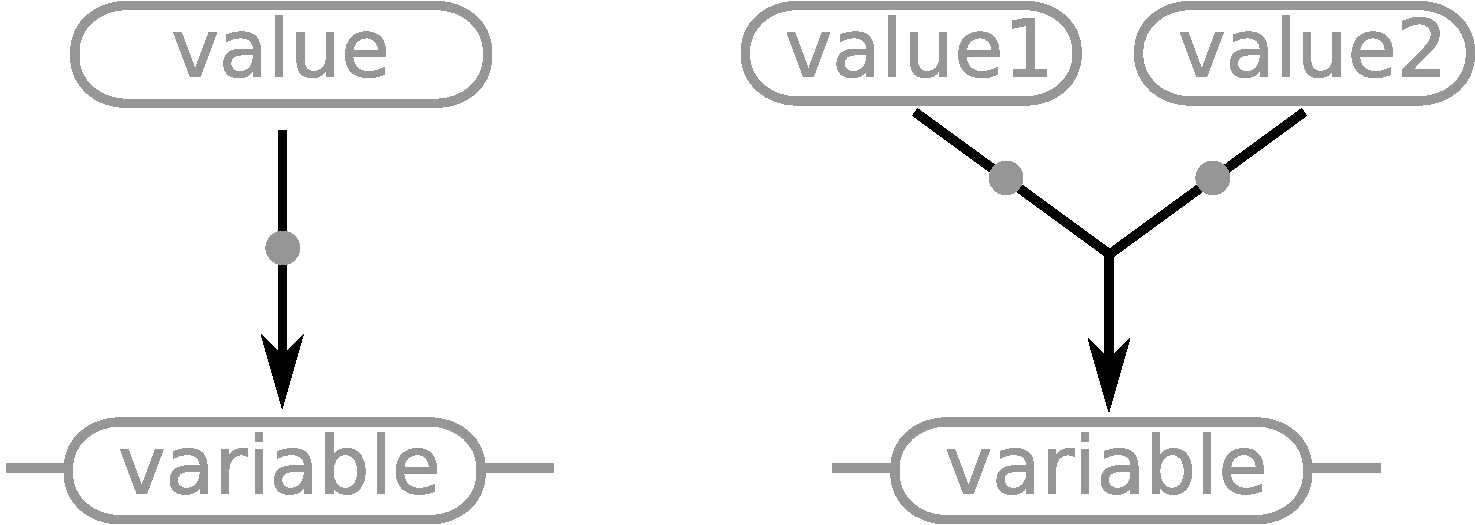
\includegraphics[scale = 0.3]{images/assignment}
  \caption{The \ER glyph for \glyph{assignment}.}
  \label{fig:assignment}
\end{figure}

\begin{figure}[H]
  \centering
  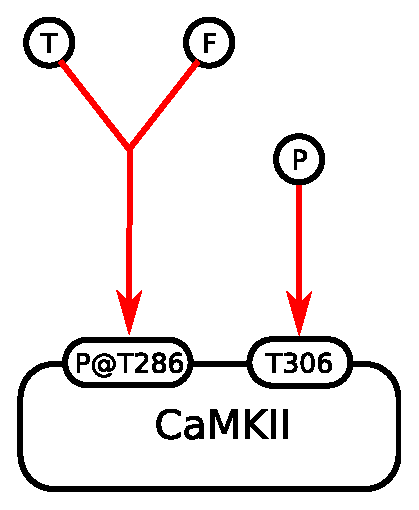
\includegraphics[scale = 0.5]{examples/ex-assignment}
  \caption{Two examples of \glyph{assignment} representing phosphorylation, by one value (phosphorylation) of a variable representing a residue, or two values (true or false) of a variable representing the phosphorylated residue.}
  \label{fig:ex-assignment}
\end{figure}


%\normalcolor
